\documentclass[journal]{IEEEtran}
% SOLARIS-Twin, journal extension of the ITEC-AP 2026 paper. Build: snakemake -c1 paper.
% Every result number is a macro from generated/macros.tex (solaris.paper.macros, results/).
\usepackage[T1]{fontenc}
\usepackage{amsmath,amssymb}
\usepackage{graphicx}
\usepackage{booktabs}
\usepackage{array}
\usepackage{cite}
\usepackage[hyphens]{url}
\usepackage[hidelinks]{hyperref}
\usepackage{textcomp}
\usepackage{siunitx}
\usepackage{tikz}
\usetikzlibrary{positioning,arrows.meta,calc,fit}
\sisetup{per-mode=symbol}
\graphicspath{{./figures/}}
% Generated by solaris.paper.macros from results/. Do not edit.
\newcommand{\BzAreaFssOne}{14.1}
\newcommand{\BzLkoIAreq}{33.4}
\newcommand{\BzLkoIDmax}{26.6}
\newcommand{\BzLkoIIAreq}{16.9}
\newcommand{\BzLkoIIDmax}{29.6}
\newcommand{\BzLkoIIchargeCut}{70}
\newcommand{\BzLkoIIcharges}{8}
\newcommand{\BzLkoIIchargesNoSolar}{27}
\newcommand{\BzLkoIIclass}{moderately solar-assisted}
\newcommand{\BzLkoIIdemand}{4{,}976}
\newcommand{\BzLkoIIfss}{0.713}
\newcommand{\BzLkoIIfssSyn}{0.77}
\newcommand{\BzLkoIIfssTwo}{0.71}
\newcommand{\BzLkoIIgrid}{1{,}422}
\newcommand{\BzLkoIIpayFull}{39.2}
\newcommand{\BzLkoIIpayPV}{18.3}
\newcommand{\BzLkoIIrelief}{71}
\newcommand{\BzLkoIchargeCut}{34}
\newcommand{\BzLkoIcharges}{35}
\newcommand{\BzLkoIchargesNoSolar}{53}
\newcommand{\BzLkoIclass}{grid-dependent}
\newcommand{\BzLkoIdemand}{9{,}817}
\newcommand{\BzLkoIfss}{0.363}
\newcommand{\BzLkoIfssSyn}{0.39}
\newcommand{\BzLkoIfssTwo}{0.36}
\newcommand{\BzLkoIgrid}{6{,}272}
\newcommand{\BzLkoIpayFull}{39.0}
\newcommand{\BzLkoIpayPV}{18.2}
\newcommand{\BzLkoIrelief}{36}
\newcommand{\BzLkoTmean}{26.8}
\newcommand{\BzLkoghi}{1843.6}
\newcommand{\BzLkopsh}{5.05}
\newcommand{\BzLonIAreq}{50.2}
\newcommand{\BzLonIDmax}{18.7}
\newcommand{\BzLonIIAreq}{23.9}
\newcommand{\BzLonIIDmax}{20.5}
\newcommand{\BzLonIIchargeCut}{50}
\newcommand{\BzLonIIcharges}{12}
\newcommand{\BzLonIIchargesNoSolar}{24}
\newcommand{\BzLonIIclass}{moderately solar-assisted}
\newcommand{\BzLonIIdemand}{4{,}404}
\newcommand{\BzLonIIfss}{0.517}
\newcommand{\BzLonIIfssSyn}{0.51}
\newcommand{\BzLonIIfssTwo}{0.52}
\newcommand{\BzLonIIgrid}{2{,}122}
\newcommand{\BzLonIIpayFull}{11.9}
\newcommand{\BzLonIIpayPV}{5.6}
\newcommand{\BzLonIIrelief}{52}
\newcommand{\BzLonIchargeCut}{22}
\newcommand{\BzLonIcharges}{39}
\newcommand{\BzLonIchargesNoSolar}{50}
\newcommand{\BzLonIclass}{grid-dependent}
\newcommand{\BzLonIdemand}{9{,}250}
\newcommand{\BzLonIfss}{0.248}
\newcommand{\BzLonIfssSyn}{0.24}
\newcommand{\BzLonIfssTwo}{0.25}
\newcommand{\BzLonIgrid}{6{,}982}
\newcommand{\BzLonIpayFull}{11.9}
\newcommand{\BzLonIpayPV}{5.5}
\newcommand{\BzLonIrelief}{25}
\newcommand{\BzLonTmean}{11.1}
\newcommand{\BzLonghi}{1050.7}
\newcommand{\BzLonpsh}{2.88}
\newcommand{\BzPhxIAreq}{28.8}
\newcommand{\BzPhxIDmax}{33.6}
\newcommand{\BzPhxIIAreq}{14.4}
\newcommand{\BzPhxIIDmax}{37.5}
\newcommand{\BzPhxIIchargeCut}{81}
\newcommand{\BzPhxIIcharges}{5}
\newcommand{\BzPhxIIchargesNoSolar}{27}
\newcommand{\BzPhxIIclass}{highly solar-assisted}
\newcommand{\BzPhxIIdemand}{4{,}874}
\newcommand{\BzPhxIIfss}{0.832}
\newcommand{\BzPhxIIfssSyn}{0.94}
\newcommand{\BzPhxIIfssTwo}{0.83}
\newcommand{\BzPhxIIgrid}{885}
\newcommand{\BzPhxIIpayFull}{15.2}
\newcommand{\BzPhxIIpayPV}{7.1}
\newcommand{\BzPhxIIrelief}{82}
\newcommand{\BzPhxIchargeCut}{43}
\newcommand{\BzPhxIcharges}{31}
\newcommand{\BzPhxIchargesNoSolar}{54}
\newcommand{\BzPhxIclass}{grid-dependent}
\newcommand{\BzPhxIdemand}{9{,}716}
\newcommand{\BzPhxIfss}{0.419}
\newcommand{\BzPhxIfssSyn}{0.47}
\newcommand{\BzPhxIfssTwo}{0.42}
\newcommand{\BzPhxIgrid}{5{,}541}
\newcommand{\BzPhxIpayFull}{14.9}
\newcommand{\BzPhxIpayPV}{7.0}
\newcommand{\BzPhxIrelief}{42}
\newcommand{\BzPhxTmean}{23.2}
\newcommand{\BzPhxghi}{2110.0}
\newcommand{\BzPhxpsh}{5.78}
\newcommand{\BzRelHi}{0.840}
\newcommand{\BzRelLo}{0.832}
\newcommand{\BzWhkmCity}{210}
\newcommand{\BzWhkmFull}{237}
\newcommand{\EeightAgree}{99.1}
\newcommand{\EeightBandDis}{65}
\newcommand{\EeightBandShare}{3.2}
\newcommand{\EeightBeyondAgree}{99.7}
\newcommand{\EeightBeyondMaxPp}{0.65}
\newcommand{\EeightEmbreeAgree}{99.99}
\newcommand{\EeightEmbreeMaxPp}{0.02}
\newcommand{\EeightMarksMax}{0.14}
\newcommand{\EeightMarksN}{5}
\newcommand{\EeightMaxPp}{2.37}
\newcommand{\EeightMeanPp}{0.38}
\newcommand{\EeightRecords}{15.5}
\newcommand{\EeightSvfAllMae}{0.171}
\newcommand{\EeightSvfAllN}{8}
\newcommand{\EeightSvfAllR}{0.29}
\newcommand{\EeightSvfAllRmse}{0.360}
\newcommand{\EeightSvfKeptMae}{0.054}
\newcommand{\EeightSvfKeptN}{7}
\newcommand{\EeightSvfKeptR}{0.92}
\newcommand{\EeightSvfKeptRmse}{0.088}
\newcommand{\EeightTrips}{120}
\newcommand{\EeightWithin}{119}
\newcommand{\EfiveAFourBZero}{0.419}
\newcommand{\EfiveAFourBZeroCharges}{31}
\newcommand{\EfiveAFourBZeroGrid}{5{,}541}
\newcommand{\EfiveAFourBZeroRelief}{42}
\newcommand{\EfiveAFourBuildings}{0.262}
\newcommand{\EfiveAFourBuildingsCharges}{40}
\newcommand{\EfiveAFourBuildingsDelta}{\textminus{}0.009}
\newcommand{\EfiveAFourBuildingsDrop}{0.009}
\newcommand{\EfiveAFourBuildingsGrid}{7{,}076}
\newcommand{\EfiveAFourBuildingsRelief}{26}
\newcommand{\EfiveAFourChain}{0.425}
\newcommand{\EfiveAFourChainCharges}{32}
\newcommand{\EfiveAFourChainDelta}{0.004}
\newcommand{\EfiveAFourChainDrop}{\textminus{}0.004}
\newcommand{\EfiveAFourChainGrid}{5{,}652}
\newcommand{\EfiveAFourChainRelief}{42}
\newcommand{\EfiveAFourFacets}{0.345}
\newcommand{\EfiveAFourFacetsCharges}{36}
\newcommand{\EfiveAFourFacetsDelta}{\textminus{}0.079}
\newcommand{\EfiveAFourFacetsDrop}{0.079}
\newcommand{\EfiveAFourFacetsGrid}{6{,}352}
\newcommand{\EfiveAFourFacetsRelief}{35}
\newcommand{\EfiveAFourLoss}{39}
\newcommand{\EfiveAFourMismatch}{0.257}
\newcommand{\EfiveAFourMismatchCharges}{41}
\newcommand{\EfiveAFourMismatchDelta}{\textminus{}0.004}
\newcommand{\EfiveAFourMismatchDrop}{0.004}
\newcommand{\EfiveAFourMismatchGrid}{7{,}251}
\newcommand{\EfiveAFourMismatchRelief}{26}
\newcommand{\EfiveAFourParking}{0.271}
\newcommand{\EfiveAFourParkingCharges}{40}
\newcommand{\EfiveAFourParkingDelta}{\textminus{}0.074}
\newcommand{\EfiveAFourParkingDrop}{0.074}
\newcommand{\EfiveAFourParkingGrid}{7{,}067}
\newcommand{\EfiveAFourParkingRelief}{27}
\newcommand{\EfiveAFourSchedule}{0.421}
\newcommand{\EfiveAFourScheduleCharges}{32}
\newcommand{\EfiveAFourScheduleDelta}{0.002}
\newcommand{\EfiveAFourScheduleDrop}{\textminus{}0.002}
\newcommand{\EfiveAFourScheduleGrid}{5{,}650}
\newcommand{\EfiveAFourScheduleRelief}{42}
\newcommand{\EfiveAFourTrees}{0.261}
\newcommand{\EfiveAFourTreesCharges}{40}
\newcommand{\EfiveAFourTreesDelta}{\textminus{}0.001}
\newcommand{\EfiveAFourTreesDrop}{0.001}
\newcommand{\EfiveAFourTreesGrid}{7{,}066}
\newcommand{\EfiveAFourTreesRelief}{26}
\newcommand{\EfiveAOneBZero}{0.832}
\newcommand{\EfiveAOneBZeroCharges}{5}
\newcommand{\EfiveAOneBZeroGrid}{885}
\newcommand{\EfiveAOneBZeroRelief}{82}
\newcommand{\EfiveAOneBuildings}{0.543}
\newcommand{\EfiveAOneBuildingsCharges}{12}
\newcommand{\EfiveAOneBuildingsDelta}{\textminus{}0.009}
\newcommand{\EfiveAOneBuildingsDrop}{0.009}
\newcommand{\EfiveAOneBuildingsGrid}{2{,}126}
\newcommand{\EfiveAOneBuildingsRelief}{54}
\newcommand{\EfiveAOneChain}{0.835}
\newcommand{\EfiveAOneChainCharges}{4}
\newcommand{\EfiveAOneChainDelta}{0.002}
\newcommand{\EfiveAOneChainDrop}{\textminus{}0.002}
\newcommand{\EfiveAOneChainGrid}{710}
\newcommand{\EfiveAOneChainRelief}{84}
\newcommand{\EfiveAOneFacets}{0.677}
\newcommand{\EfiveAOneFacetsCharges}{9}
\newcommand{\EfiveAOneFacetsDelta}{\textminus{}0.159}
\newcommand{\EfiveAOneFacetsDrop}{0.159}
\newcommand{\EfiveAOneFacetsGrid}{1{,}594}
\newcommand{\EfiveAOneFacetsRelief}{68}
\newcommand{\EfiveAOneLoss}{38}
\newcommand{\EfiveAOneMismatch}{0.512}
\newcommand{\EfiveAOneMismatchCharges}{13}
\newcommand{\EfiveAOneMismatchDelta}{\textminus{}0.030}
\newcommand{\EfiveAOneMismatchDrop}{0.030}
\newcommand{\EfiveAOneMismatchGrid}{2{,}300}
\newcommand{\EfiveAOneMismatchRelief}{51}
\newcommand{\EfiveAOneParking}{0.552}
\newcommand{\EfiveAOneParkingCharges}{12}
\newcommand{\EfiveAOneParkingDelta}{\textminus{}0.125}
\newcommand{\EfiveAOneParkingDrop}{0.125}
\newcommand{\EfiveAOneParkingGrid}{2{,}118}
\newcommand{\EfiveAOneParkingRelief}{55}
\newcommand{\EfiveAOneResEffect}{0.001}
\newcommand{\EfiveAOneSchedule}{0.833}
\newcommand{\EfiveAOneScheduleCharges}{5}
\newcommand{\EfiveAOneScheduleDelta}{0.001}
\newcommand{\EfiveAOneScheduleDrop}{\textminus{}0.001}
\newcommand{\EfiveAOneScheduleGrid}{883}
\newcommand{\EfiveAOneScheduleRelief}{82}
\newcommand{\EfiveAOneTrees}{0.542}
\newcommand{\EfiveAOneTreesCharges}{13}
\newcommand{\EfiveAOneTreesDelta}{\textminus{}0.001}
\newcommand{\EfiveAOneTreesDrop}{0.001}
\newcommand{\EfiveAOneTreesGrid}{2{,}306}
\newcommand{\EfiveAOneTreesRelief}{54}
\newcommand{\EfiveAOneYearEffect}{0.004}
\newcommand{\EfiveAThreeBZero}{0.832}
\newcommand{\EfiveAThreeBZeroCharges}{5}
\newcommand{\EfiveAThreeBZeroGrid}{885}
\newcommand{\EfiveAThreeBZeroRelief}{82}
\newcommand{\EfiveAThreeBuildings}{0.403}
\newcommand{\EfiveAThreeBuildingsCharges}{16}
\newcommand{\EfiveAThreeBuildingsDelta}{\textminus{}0.017}
\newcommand{\EfiveAThreeBuildingsDrop}{0.017}
\newcommand{\EfiveAThreeBuildingsGrid}{2{,}835}
\newcommand{\EfiveAThreeBuildingsRelief}{40}
\newcommand{\EfiveAThreeChain}{0.835}
\newcommand{\EfiveAThreeChainCharges}{4}
\newcommand{\EfiveAThreeChainDelta}{0.002}
\newcommand{\EfiveAThreeChainDrop}{\textminus{}0.002}
\newcommand{\EfiveAThreeChainGrid}{710}
\newcommand{\EfiveAThreeChainRelief}{84}
\newcommand{\EfiveAThreeFacets}{0.676}
\newcommand{\EfiveAThreeFacetsCharges}{9}
\newcommand{\EfiveAThreeFacetsDelta}{\textminus{}0.160}
\newcommand{\EfiveAThreeFacetsDrop}{0.160}
\newcommand{\EfiveAThreeFacetsGrid}{1{,}588}
\newcommand{\EfiveAThreeFacetsRelief}{68}
\newcommand{\EfiveAThreeLoss}{60}
\newcommand{\EfiveAThreeMismatch}{0.335}
\newcommand{\EfiveAThreeMismatchCharges}{18}
\newcommand{\EfiveAThreeMismatchDelta}{\textminus{}0.067}
\newcommand{\EfiveAThreeMismatchDrop}{0.067}
\newcommand{\EfiveAThreeMismatchGrid}{3{,}172}
\newcommand{\EfiveAThreeMismatchRelief}{33}
\newcommand{\EfiveAThreeParking}{0.420}
\newcommand{\EfiveAThreeParkingCharges}{16}
\newcommand{\EfiveAThreeParkingDelta}{\textminus{}0.256}
\newcommand{\EfiveAThreeParkingDrop}{0.256}
\newcommand{\EfiveAThreeParkingGrid}{2{,}823}
\newcommand{\EfiveAThreeParkingRelief}{42}
\newcommand{\EfiveAThreeSchedule}{0.833}
\newcommand{\EfiveAThreeScheduleCharges}{5}
\newcommand{\EfiveAThreeScheduleDelta}{0.001}
\newcommand{\EfiveAThreeScheduleDrop}{\textminus{}0.001}
\newcommand{\EfiveAThreeScheduleGrid}{883}
\newcommand{\EfiveAThreeScheduleRelief}{82}
\newcommand{\EfiveAThreeTrees}{0.402}
\newcommand{\EfiveAThreeTreesCharges}{16}
\newcommand{\EfiveAThreeTreesDelta}{\textminus{}0.001}
\newcommand{\EfiveAThreeTreesDrop}{0.001}
\newcommand{\EfiveAThreeTreesGrid}{2{,}839}
\newcommand{\EfiveAThreeTreesRelief}{40}
\newcommand{\EfiveATwoBZero}{0.832}
\newcommand{\EfiveATwoBZeroCharges}{5}
\newcommand{\EfiveATwoBZeroGrid}{885}
\newcommand{\EfiveATwoBZeroRelief}{82}
\newcommand{\EfiveATwoBuildings}{0.291}
\newcommand{\EfiveATwoBuildingsCharges}{19}
\newcommand{\EfiveATwoBuildingsDelta}{\textminus{}0.017}
\newcommand{\EfiveATwoBuildingsDrop}{0.017}
\newcommand{\EfiveATwoBuildingsGrid}{3{,}369}
\newcommand{\EfiveATwoBuildingsRelief}{29}
\newcommand{\EfiveATwoChain}{0.835}
\newcommand{\EfiveATwoChainCharges}{4}
\newcommand{\EfiveATwoChainDelta}{0.002}
\newcommand{\EfiveATwoChainDrop}{\textminus{}0.002}
\newcommand{\EfiveATwoChainGrid}{710}
\newcommand{\EfiveATwoChainRelief}{84}
\newcommand{\EfiveATwoFacets}{0.678}
\newcommand{\EfiveATwoFacetsCharges}{9}
\newcommand{\EfiveATwoFacetsDelta}{\textminus{}0.158}
\newcommand{\EfiveATwoFacetsDrop}{0.158}
\newcommand{\EfiveATwoFacetsGrid}{1{,}593}
\newcommand{\EfiveATwoFacetsRelief}{68}
\newcommand{\EfiveATwoLoss}{69}
\newcommand{\EfiveATwoMismatch}{0.256}
\newcommand{\EfiveATwoMismatchCharges}{20}
\newcommand{\EfiveATwoMismatchDelta}{\textminus{}0.034}
\newcommand{\EfiveATwoMismatchDrop}{0.034}
\newcommand{\EfiveATwoMismatchGrid}{3{,}540}
\newcommand{\EfiveATwoMismatchRelief}{26}
\newcommand{\EfiveATwoParking}{0.308}
\newcommand{\EfiveATwoParkingCharges}{20}
\newcommand{\EfiveATwoParkingDelta}{\textminus{}0.369}
\newcommand{\EfiveATwoParkingDrop}{0.369}
\newcommand{\EfiveATwoParkingGrid}{3{,}524}
\newcommand{\EfiveATwoParkingRelief}{31}
\newcommand{\EfiveATwoResEffect}{0.001}
\newcommand{\EfiveATwoSchedule}{0.833}
\newcommand{\EfiveATwoScheduleCharges}{5}
\newcommand{\EfiveATwoScheduleDelta}{0.001}
\newcommand{\EfiveATwoScheduleDrop}{\textminus{}0.001}
\newcommand{\EfiveATwoScheduleGrid}{883}
\newcommand{\EfiveATwoScheduleRelief}{82}
\newcommand{\EfiveATwoTrees}{0.290}
\newcommand{\EfiveATwoTreesCharges}{19}
\newcommand{\EfiveATwoTreesDelta}{\textminus{}0.001}
\newcommand{\EfiveATwoTreesDrop}{0.001}
\newcommand{\EfiveATwoTreesGrid}{3{,}368}
\newcommand{\EfiveATwoTreesRelief}{29}
\newcommand{\EfiveATwoYearEffect}{0.002}
\newcommand{\EfiveBalance}{\ensuremath{1\times10^{-14}}}
\newcommand{\EfourPFive}{0.64}
\newcommand{\EfourPFour}{0.88}
\newcommand{\EfourPOne}{0.94}
\newcommand{\EfourPThree}{0.45}
\newcommand{\EfourPTwo}{0.32}
\newcommand{\EfourSolweigLo}{96.7}
\newcommand{\EoneBeam}{99.6}
\newcommand{\EoneDsvf}{0.008}
\newcommand{\EonePassed}{40}
\newcommand{\EoneSolweigHi}{99.3}
\newcommand{\EoneSolweigLo}{98.0}
\newcommand{\EoneTotal}{40}
\newcommand{\EsevenAFourAreq}{48.8}
\newcommand{\EsevenAFourAsim}{48.9}
\newcommand{\EsevenAFourDmax}{15.5}
\newcommand{\EsevenAFourErr}{\textminus{}0.3}
\newcommand{\EsevenAFourFullSkinBaseHi}{0.26}
\newcommand{\EsevenAFourFullSkinBaseLo}{0.20}
\newcommand{\EsevenAFourFullSkinFchain}{1.01}
\newcommand{\EsevenAFourFullSkinFgeo}{0.81}
\newcommand{\EsevenAFourFullSkinFmm}{0.98}
\newcommand{\EsevenAFourFullSkinFsh}{0.74}
\newcommand{\EsevenAFourFullSkinMaxHi}{0.43}
\newcommand{\EsevenAFourFullSkinMaxLo}{0.33}
\newcommand{\EsevenAFourRoofBaseHi}{0.33}
\newcommand{\EsevenAFourRoofBaseLo}{0.25}
\newcommand{\EsevenAFourRoofFchain}{1.01}
\newcommand{\EsevenAFourRoofFgeo}{1.00}
\newcommand{\EsevenAFourRoofFmm}{0.98}
\newcommand{\EsevenAFourRoofFsh}{0.78}
\newcommand{\EsevenAFourRoofHoodBaseHi}{0.33}
\newcommand{\EsevenAFourRoofHoodBaseLo}{0.25}
\newcommand{\EsevenAFourRoofHoodFchain}{1.01}
\newcommand{\EsevenAFourRoofHoodFgeo}{0.99}
\newcommand{\EsevenAFourRoofHoodFmm}{0.98}
\newcommand{\EsevenAFourRoofHoodFsh}{0.78}
\newcommand{\EsevenAFourRoofHoodMaxHi}{0.55}
\newcommand{\EsevenAFourRoofHoodMaxLo}{0.42}
\newcommand{\EsevenAFourRoofMaxHi}{0.55}
\newcommand{\EsevenAFourRoofMaxLo}{0.42}
\newcommand{\EsevenAOneAreq}{24.1}
\newcommand{\EsevenAOneAsim}{23.6}
\newcommand{\EsevenAOneDmax}{17.8}
\newcommand{\EsevenAOneErr}{2.1}
\newcommand{\EsevenAOneFullSkinBaseHi}{0.51}
\newcommand{\EsevenAOneFullSkinBaseLo}{0.39}
\newcommand{\EsevenAOneFullSkinFchain}{1.00}
\newcommand{\EsevenAOneFullSkinFgeo}{0.80}
\newcommand{\EsevenAOneFullSkinFmm}{0.94}
\newcommand{\EsevenAOneFullSkinFsh}{0.79}
\newcommand{\EsevenAOneFullSkinMaxHi}{0.86}
\newcommand{\EsevenAOneFullSkinMaxLo}{0.65}
\newcommand{\EsevenAOneRoofBaseHi}{0.66}
\newcommand{\EsevenAOneRoofBaseLo}{0.50}
\newcommand{\EsevenAOneRoofFchain}{1.00}
\newcommand{\EsevenAOneRoofFgeo}{1.00}
\newcommand{\EsevenAOneRoofFmm}{0.93}
\newcommand{\EsevenAOneRoofFsh}{0.84}
\newcommand{\EsevenAOneRoofHoodBaseHi}{0.66}
\newcommand{\EsevenAOneRoofHoodBaseLo}{0.50}
\newcommand{\EsevenAOneRoofHoodFchain}{1.00}
\newcommand{\EsevenAOneRoofHoodFgeo}{1.00}
\newcommand{\EsevenAOneRoofHoodFmm}{0.94}
\newcommand{\EsevenAOneRoofHoodFsh}{0.83}
\newcommand{\EsevenAOneRoofHoodMaxHi}{1.10}
\newcommand{\EsevenAOneRoofHoodMaxLo}{0.83}
\newcommand{\EsevenAOneRoofMaxHi}{1.11}
\newcommand{\EsevenAOneRoofMaxLo}{0.84}
\newcommand{\EsevenAThreeAreq}{38.0}
\newcommand{\EsevenAThreeAsim}{37.7}
\newcommand{\EsevenAThreeDmax}{6.8}
\newcommand{\EsevenAThreeErr}{0.8}
\newcommand{\EsevenAThreeFullSkinBaseHi}{0.33}
\newcommand{\EsevenAThreeFullSkinBaseLo}{0.26}
\newcommand{\EsevenAThreeFullSkinFchain}{1.00}
\newcommand{\EsevenAThreeFullSkinFgeo}{0.80}
\newcommand{\EsevenAThreeFullSkinFmm}{0.82}
\newcommand{\EsevenAThreeFullSkinFsh}{0.58}
\newcommand{\EsevenAThreeFullSkinMaxHi}{0.55}
\newcommand{\EsevenAThreeFullSkinMaxLo}{0.42}
\newcommand{\EsevenAThreeRoofBaseHi}{0.31}
\newcommand{\EsevenAThreeRoofBaseLo}{0.24}
\newcommand{\EsevenAThreeRoofFchain}{1.00}
\newcommand{\EsevenAThreeRoofFgeo}{1.00}
\newcommand{\EsevenAThreeRoofFmm}{0.71}
\newcommand{\EsevenAThreeRoofFsh}{0.50}
\newcommand{\EsevenAThreeRoofHoodBaseHi}{0.34}
\newcommand{\EsevenAThreeRoofHoodBaseLo}{0.26}
\newcommand{\EsevenAThreeRoofHoodFchain}{1.00}
\newcommand{\EsevenAThreeRoofHoodFgeo}{1.00}
\newcommand{\EsevenAThreeRoofHoodFmm}{0.75}
\newcommand{\EsevenAThreeRoofHoodFsh}{0.52}
\newcommand{\EsevenAThreeRoofHoodMaxHi}{0.56}
\newcommand{\EsevenAThreeRoofHoodMaxLo}{0.43}
\newcommand{\EsevenAThreeRoofMaxHi}{0.51}
\newcommand{\EsevenAThreeRoofMaxLo}{0.39}
\newcommand{\EsevenATwoAreq}{51.3}
\newcommand{\EsevenATwoAsim}{51.5}
\newcommand{\EsevenATwoDmax}{1.9}
\newcommand{\EsevenATwoErr}{\textminus{}0.5}
\newcommand{\EsevenATwoFullSkinBaseHi}{0.26}
\newcommand{\EsevenATwoFullSkinBaseLo}{0.20}
\newcommand{\EsevenATwoFullSkinFchain}{1.00}
\newcommand{\EsevenATwoFullSkinFgeo}{0.80}
\newcommand{\EsevenATwoFullSkinFmm}{0.87}
\newcommand{\EsevenATwoFullSkinFsh}{0.40}
\newcommand{\EsevenATwoFullSkinMaxHi}{0.42}
\newcommand{\EsevenATwoFullSkinMaxLo}{0.32}
\newcommand{\EsevenATwoRoofBaseHi}{0.33}
\newcommand{\EsevenATwoRoofBaseLo}{0.25}
\newcommand{\EsevenATwoRoofFchain}{1.00}
\newcommand{\EsevenATwoRoofFgeo}{1.00}
\newcommand{\EsevenATwoRoofFmm}{0.84}
\newcommand{\EsevenATwoRoofFsh}{0.44}
\newcommand{\EsevenATwoRoofHoodBaseHi}{0.32}
\newcommand{\EsevenATwoRoofHoodBaseLo}{0.25}
\newcommand{\EsevenATwoRoofHoodFchain}{1.00}
\newcommand{\EsevenATwoRoofHoodFgeo}{1.00}
\newcommand{\EsevenATwoRoofHoodFmm}{0.86}
\newcommand{\EsevenATwoRoofHoodFsh}{0.43}
\newcommand{\EsevenATwoRoofHoodMaxHi}{0.53}
\newcommand{\EsevenATwoRoofHoodMaxLo}{0.41}
\newcommand{\EsevenATwoRoofMaxHi}{0.54}
\newcommand{\EsevenATwoRoofMaxLo}{0.41}
\newcommand{\EsevenMaxErr}{2.6}
\newcommand{\EsevenMaxErrFixed}{3.3}
\newcommand{\EsevenN}{60}
\newcommand{\EsixAlpha}{0.46}
\newcommand{\EsixBeta}{0.58}
\newcommand{\EsixDriving}{0.96}
\newcommand{\EsixK}{1.49}
\newcommand{\EsixParking}{0.73}
\newcommand{\EsixPthreeHi}{0.73}
\newcommand{\EsixPthreeLo}{0.56}
\newcommand{\EsixPtwo}{0.96}
\newcommand{\EsixRsq}{0.84}
\newcommand{\EsixUniform}{\ensuremath{7\times10^{-5}}}
\newcommand{\EthreeDenseB}{0.72}
\newcommand{\EthreeDenseBShaded}{32}
\newcommand{\EthreeDenseCZeroOne}{0.71}
\newcommand{\EthreeDenseCZeroOneShaded}{32}
\newcommand{\EthreeDenseCZeroThree}{0.72}
\newcommand{\EthreeDenseCZeroThreeShaded}{32}
\newcommand{\EthreeDenseCZeroZeroThree}{0.71}
\newcommand{\EthreeDenseCZeroZeroThreeShaded}{32}
\newcommand{\EthreeMixedB}{0.90}
\newcommand{\EthreeMixedBShaded}{11}
\newcommand{\EthreeMixedCZeroOne}{0.90}
\newcommand{\EthreeMixedCZeroOneShaded}{12}
\newcommand{\EthreeMixedCZeroThree}{0.90}
\newcommand{\EthreeMixedCZeroThreeShaded}{12}
\newcommand{\EthreeMixedCZeroZeroThree}{0.89}
\newcommand{\EthreeMixedCZeroZeroThreeShaded}{12}
\newcommand{\EthreeOpenB}{0.93}
\newcommand{\EthreeOpenBShaded}{7}
\newcommand{\EthreeOpenCZeroOne}{0.92}
\newcommand{\EthreeOpenCZeroOneShaded}{10}
\newcommand{\EthreeOpenCZeroThree}{0.92}
\newcommand{\EthreeOpenCZeroThreeShaded}{9}
\newcommand{\EthreeOpenCZeroZeroThree}{0.91}
\newcommand{\EthreeOpenCZeroZeroThreeShaded}{10}
\newcommand{\EthreeTrips}{360}
\newcommand{\EtwoFgeo}{0.805}
\newcommand{\EtwoFgeoRoof}{0.380}
\newcommand{\EtwoIChargesTwoa}{31}
\newcommand{\EtwoIChargesTwoc}{36}
\newcommand{\EtwoIChargesTwod}{45}
\newcommand{\EtwoIGate}{\textminus{}0.03}
\newcommand{\EtwoIIChargesTwoa}{5}
\newcommand{\EtwoIIChargesTwoc}{9}
\newcommand{\EtwoIIChargesTwod}{18}
\newcommand{\EtwoIIGate}{\textminus{}0.03}
\newcommand{\EtwoIIThermal}{0.55}
\newcommand{\EtwoIITwoa}{0.832}
\newcommand{\EtwoIITwob}{0.832}
\newcommand{\EtwoIITwobF}{0.836}
\newcommand{\EtwoIITwoc}{0.678}
\newcommand{\EtwoIITwod}{0.335}
\newcommand{\EtwoIThermal}{0.60}
\newcommand{\EtwoITwoa}{0.419}
\newcommand{\EtwoITwob}{0.419}
\newcommand{\EtwoITwobF}{0.421}
\newcommand{\EtwoITwoc}{0.342}
\newcommand{\EtwoITwod}{0.170}
\newcommand{\FacetHoodGhi}{0.99}
\newcommand{\FacetRoofGhi}{1.00}
\newcommand{\FacetSideLeftGhi}{0.56}
\newcommand{\FacetSideRightGhi}{0.56}
\newcommand{\FacetTailgateGhi}{0.74}
\newcommand{\FreshAdded}{14}
\newcommand{\FreshCandidates}{159}
\newcommand{\FreshDemolished}{12}
\newcommand{\FreshRejected}{19}
\newcommand{\FreshReviewed}{45}
\newcommand{\FreshUnreviewed}{114}
\newcommand{\GapLkoDistribution}{0.027}
\newcommand{\GapLkoMagnitude}{0.030}
\newcommand{\GapLkoTotal}{0.058}
\newcommand{\GapLonDistribution}{0.022}
\newcommand{\GapLonMagnitude}{\textminus{}0.030}
\newcommand{\GapLonTotal}{\textminus{}0.009}
\newcommand{\GapPhxDistribution}{0.047}
\newcommand{\GapPhxMagnitude}{0.058}
\newcommand{\GapPhxTotal}{0.106}
\newcommand{\GeoArea}{238}
\newcommand{\GeoDensity}{22.2}
\newcommand{\GeoHoles}{0.75}
\newcommand{\GeoMarkMad}{0.14}
\newcommand{\GeoMarkMedian}{\textminus{}0.11}
\newcommand{\GeoMarkWithin}{69}
\newcommand{\GeoMarks}{87}
\newcommand{\GeoOverture}{135{,}145}
\newcommand{\GeoPctBuilding}{23.9}
\newcommand{\GeoPctGround}{71.6}
\newcommand{\GeoPctTree}{4.4}
\newcommand{\GeoPoints}{5.28}
\newcommand{\GeoTiles}{952}
\newcommand{\PsixTraces}{120}
\newcommand{\RouteCandidates}{128}
\newcommand{\RouteDenseLen}{7.8}
\newcommand{\RouteDenseSvf}{0.74}
\newcommand{\RouteMixedLen}{7.8}
\newcommand{\RouteMixedSvf}{0.90}
\newcommand{\RouteOpenLen}{8.3}
\newcommand{\RouteOpenSvf}{0.96}
\newcommand{\SitePFiveSvf}{0.95}
\newcommand{\SitePFourSvf}{0.91}
\newcommand{\SitePOneSvf}{0.95}
\newcommand{\SitePThreeSvf}{0.48}
\newcommand{\SitePTwoSvf}{0.34}
\newcommand{\WxFiveCell}{518064}
\newcommand{\WxFiveGhi}{2132.9}
\newcommand{\WxTmyCell}{323705}
\newcommand{\WxTmyGhi}{2110.0}
\newcommand{\WxZenithFive}{0.06}
\newcommand{\WxZenithTmy}{0.24}

\newcommand{\fss}{f_{\mathrm{ss}}}
\newcommand{\Fgeo}{F_{\mathrm{geo}}}
\newcommand{\Fsh}{F_{\mathrm{sh}}}
\newcommand{\Fmm}{F_{\mathrm{mm}}}
\newcommand{\Fpark}{F_{\mathrm{park}}}
\newcommand{\todo}[1]{\textbf{[#1]}}

\begin{document}

\title{A Digital Twin for Shading-Aware Assessment of Vehicle-Integrated Photovoltaics on a Heavy Electric Vehicle}

\author{Aditya~Kumar, Anandsagar~Gaikwad, and Arjun~Deo%
\thanks{This work extends the paper ``SOLARIS: A first-principles, drive-cycle- and climate-resolved methodology and open toolkit for assessing solar-assisted heavy electric vehicles,'' accepted for presentation at the IEEE Transportation Electrification Conference and Expo, Asia-Pacific (ITEC-AP 2026), Busan, Republic of Korea, 1--4 December 2026~\cite{ref_conf}.}%
\thanks{A. Kumar and A. Gaikwad are with the Department of Computer Science and Engineering, Rajiv Gandhi Institute of Petroleum Technology, Jais, Amethi, Uttar Pradesh, India (e-mail: 23cs2006@rgipt.ac.in; 23cs3008@rgipt.ac.in). A. Deo is with the Rajiv Gandhi Institute of Petroleum Technology, Bengaluru Campus, Karnataka, India (e-mail: arjund@rgipt.ac.in).}%
\thanks{Corresponding author: Aditya Kumar, \todo{postal address}, \todo{phone}, 23cs2006@rgipt.ac.in.}}

\markboth{IEEE Transactions on Transportation Electrification}{Kumar \MakeLowercase{\textit{et al.}}: Shading-Aware Assessment of Vehicle-Integrated Photovoltaics}

\maketitle

\begin{abstract}
Feasibility studies of vehicle-integrated photovoltaics (VIPV) usually take the irradiance on a horizontal, unshaded roof. We extend SOLARIS, an hour-by-hour energy-balance toolkit for a \SI{2.5}{t} seven-seat electric vehicle, with a digital twin of central Phoenix, Arizona. The twin builds a \SI{0.5}{m} city model from \GeoPoints~billion lidar points, drives the vehicle on traffic-simulated trips along three arterials, parks it at five sites and resolves the shadow on each facet of an assumed \SI{11.6}{m^2} skin every second while driving and every five minutes while parked. On a satellite-derived typical year the conference model gives a solar self-sufficiency of \BzPhxIIfss{} at \SI{50}{km/day}. Facet orientation lowers it to \EtwoIITwoc; with parking shade, street shade and electrical mismatch, a suburban commuter ends at \EfiveAOneMismatch{} and a downtown street parker at \EfiveATwoMismatch. Most of the shading loss occurs while parked. We extend the conference design equation with orientation, shading and mismatch factors; it stays within \EsevenMaxErr\% of the full simulation. A Unity twin agrees with the Python shading engine on \EeightAgree\% of \EeightRecords~million sample-seconds. The pipeline and data recipes are open.
\end{abstract}

\begin{IEEEkeywords}
Vehicle-integrated photovoltaics, digital twin, urban shading, electric vehicles, energy self-sufficiency.
\end{IEEEkeywords}

\section{Introduction}
\IEEEPARstart{S}{olar} cells built into the body of an electric vehicle (EV) can supply part of the energy it would otherwise draw from the grid. How large that part is depends on sunlight, consumption and their timing. In an earlier paper~\cite{ref_conf} we built SOLARIS, an open toolkit that charges every harvesting component to the vehicle's mass, computes consumption on the WLTP cycle and steps the battery through a year hour by hour. For a \SI{2.5}{t} seven-seat vehicle with an \SI{11.6}{m^2} skin, satellite-derived weather gave a solar self-sufficiency $\fss$ of \BzPhxIIfssTwo{} in Phoenix, \BzLkoIIfssTwo{} in Lucknow and \BzLonIIfssTwo{} in London for \SI{50}{km/day} of urban driving.

Those numbers rest on two simplifications that most VIPV feasibility studies share. The whole skin receives global horizontal irradiance (GHI), although side panels are nearly vertical. Nothing shades the vehicle, although a car is parked for most of the day, often next to buildings or under trees, and drives through street canyons. Both make the result optimistic, and the size of the error depends on where the car is driven and parked.

This paper replaces both simplifications with a digital twin of central Phoenix and keeps the rest of the conference model unchanged, so each correction can be measured on its own. The contributions are:
\begin{enumerate}
\item a reproducible pipeline from public lidar, building and street data to a \SI{0.5}{m} city model with buildings and trees separated, checked against survey marks and updated for buildings built or demolished since the lidar flight;
\item a facet-resolved irradiance, thermal and electrical model of the vehicle skin, driven by traffic-simulated trips at \SI{1}{s} and by parking at \SI{5}{min}, with energy closure checked at every step;
\item an annual loss waterfall from the conference baseline to four daily-use archetypes, which separates the effects of facet orientation, parking shade, driving shade and electrical mismatch;
\item a shading-aware form of the conference design equation and a nomograph, checked against the full simulation;
\item a cross-check of the shading engines against an independent Unity ray-casting twin, an urban-climate model and street-level imagery.
\end{enumerate}

\section{Related Work}
Reviews of VIPV agree that yield is set by geometry, curvature, shading and climate~\cite{ref_commault,ref_samadi}. Yield models compute harvest for fleets~\cite{ref_carr} or along shaded city routes~\cite{ref_sanjose} but take the vehicle's consumption as given; power-electronics studies optimize the converter and the auxiliary battery~\cite{ref_yavasoglu}. Urban shading has been estimated from geographic data: Brito \emph{et al.}~\cite{ref_brito} found annual shading losses of up to 25\% on Lisbon roads and over 50\% at urban parking spaces, and Hoth \emph{et al.}~\cite{ref_hoth} report a median shading loss of 61\% (quartiles 38\% and 76\%) for parked cars in Berlin. San Jos\'e \emph{et al.}~\cite{ref_sanjose} recorded shadows on a driving car with a camera and showed how partial shading of cells degrades the current--voltage curve. Sky view factors (SVF) for street routing in Phoenix have been computed from synthetic fisheye images~\cite{ref_middel}, and the SOLWEIG model in UMEP~\cite{ref_solweig,ref_umep} is a standard reference for shadow patterns in urban climate work. To our knowledge no study has combined trajectory-level driving and parking shade, facet orientation and electrical mismatch with drive-cycle demand and an annual battery simulation, or done so for a heavy vehicle.

\section{Conference Baseline}
\label{sec:baseline}
The conference model~\cite{ref_conf,ref_code} is used unchanged as the reference (version~1.1.0; the refactored code reproduces every output of the conference code, as the repository tests check). Demand is the WLTP consumption at the battery, \SI{\BzWhkmCity}{Wh/km} on the city part of the cycle and \SI{\BzWhkmFull}{Wh/km} on the full cycle, plus auxiliaries and cabin cooling. Harvest is
\begin{equation}
E_{\mathrm{pv}}=A\,\eta_{\mathrm{pv}}\,\kappa_{\mathrm{pv}}\,\frac{G}{1000}\left[1+\beta(T_c-25)\right]
\label{eq:pv}
\end{equation}
with $A=\SI{11.6}{m^2}$, $\eta_{\mathrm{pv}}=0.22$, $\kappa_{\mathrm{pv}}=0.80$, $\beta=-0.4\%/\mathrm{K}$, $T_c=T_a+25G/1000$ and $G$ the GHI, plus small thermoelectric and suspension terms. The \SI{250}{kWh} pack is simulated hour by hour over a periodic year; it is recharged from 10\% to 80\% when needed. Scenario~II is \SI{50}{km/day} on the city cycle and Scenario~I \SI{100}{km/day} on the full cycle, and $\fss$ is annual harvest over annual demand. Setting harvest equal to demand gives the design area
\begin{equation}
A_{\mathrm{req}}=\frac{D\,c+E_{\mathrm{aux}}}{\eta_{\mathrm{pv}}\,\mathrm{PSH}\,\kappa_{\mathrm{pv}}\,f_T},
\label{eq:areq}
\end{equation}
where $D$ is the daily distance, $c$ the battery-side consumption, PSH the daily peak-sun hours, $f_T$ the irradiance-weighted temperature factor and $E_{\mathrm{aux}}$ the daily auxiliary energy.

Table~\ref{tab:b0} is the baseline on satellite-derived hourly typical meteorological years (TMY): NSRDB for Phoenix and Lucknow~\cite{ref_nsrdb} and PVGIS for London~\cite{ref_pvgis}. Everything that follows is for Phoenix, Scenario~II unless stated, starting from $\fss=\BzPhxIIfss$, \BzPhxIIcharges{} grid charges per year (\BzPhxIIchargesNoSolar{} without solar) and $A_{\mathrm{req}}=\SI{\BzPhxIIAreq}{m^2}$. The idealized synthetic climate of the conference paper gives \BzPhxIIfssSyn{}; of the gap of \GapPhxTotal{}, \GapPhxMagnitude{} comes from the annual irradiation and \GapPhxDistribution{} from the timing of cloud.

\begin{table}[t]
\caption{Conference Baseline on Satellite-Derived Hourly TMY (Table B0)}
\label{tab:b0}
\centering\footnotesize
\setlength{\tabcolsep}{3.2pt}
\begin{tabular}{@{}llccccc@{}}
\toprule
City & Scen. & $\fss$ & Charges/yr & Relief & $A_{\mathrm{req}}$ & $D_{\max}$ \\
 & & & (no solar) & (\%) & (\si{m^2}) & (km/day) \\
\midrule
Phoenix & II & \BzPhxIIfss & \BzPhxIIcharges{} (\BzPhxIIchargesNoSolar) & \BzPhxIIrelief & \BzPhxIIAreq & \BzPhxIIDmax \\
        & I  & \BzPhxIfss  & \BzPhxIcharges{} (\BzPhxIchargesNoSolar)   & \BzPhxIrelief  & \BzPhxIAreq  & \BzPhxIDmax \\
Lucknow & II & \BzLkoIIfss & \BzLkoIIcharges{} (\BzLkoIIchargesNoSolar) & \BzLkoIIrelief & \BzLkoIIAreq & \BzLkoIIDmax \\
        & I  & \BzLkoIfss  & \BzLkoIcharges{} (\BzLkoIchargesNoSolar)   & \BzLkoIrelief  & \BzLkoIAreq  & \BzLkoIDmax \\
London  & II & \BzLonIIfss & \BzLonIIcharges{} (\BzLonIIchargesNoSolar) & \BzLonIIrelief & \BzLonIIAreq & \BzLonIIDmax \\
        & I  & \BzLonIfss  & \BzLonIcharges{} (\BzLonIchargesNoSolar)   & \BzLonIrelief  & \BzLonIAreq  & \BzLonIDmax \\
\bottomrule
\end{tabular}\\[2pt]
{\footnotesize Relief: harvest used (harvest minus curtailment) over demand. $D_{\max}$: distance that \SI{11.6}{m^2} makes self-sufficient. TMY annual GHI \BzPhxghi, \BzLkoghi{} and \BzLonghi{} \si{kWh/m^2}.}
\end{table}

\section{Digital Twin}
\label{sec:twin}
Fig.~\ref{fig:arch} shows the twin. Python does all physics; Unity replays the same trips against the same geometry and is used only to check visibility (Section~\ref{sec:validation}). A Snakemake workflow builds every number and figure in this paper from the raw data, with fixed seeds.

\begin{figure}[t]
\centering
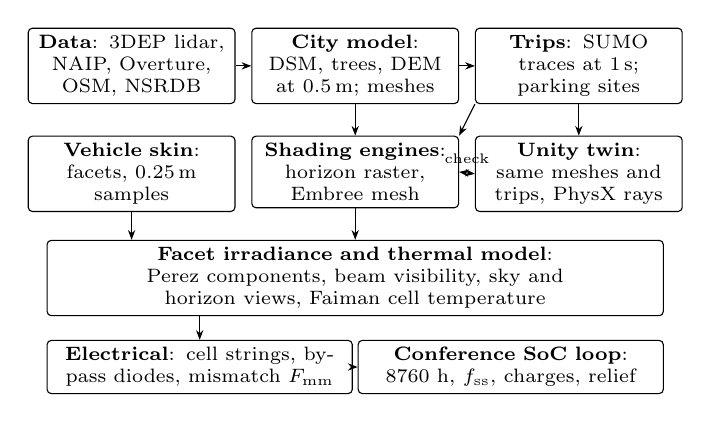
\begin{tikzpicture}[font=\scriptsize, >={Stealth[length=3.5pt]},
  box/.style={draw, rounded corners=1.5pt, align=center, inner sep=2.5pt, text width=#1},
  box/.default=2.45cm]
\node[box] (data) {\textbf{Data}: 3DEP lidar, NAIP, Overture, OSM, NSRDB};
\node[box, right=2mm of data] (geo) {\textbf{City model}: DSM, trees, DEM at \SI{0.5}{m}; meshes};
\node[box, right=2mm of geo] (traj) {\textbf{Trips}: SUMO traces at \SI{1}{s}; parking sites};
\node[box, below=4mm of geo] (shade) {\textbf{Shading engines}: horizon raster, Embree mesh};
\node[box, below=4mm of data] (veh) {\textbf{Vehicle skin}: facets, \SI{0.25}{m} samples};
\node[box, below=4mm of traj] (unity) {\textbf{Unity twin}: same meshes and trips, PhysX rays};
\node[box=7.65cm, below=4mm of shade] (irr) {\textbf{Facet irradiance and thermal model}: Perez components, beam visibility, sky and horizon views, Faiman cell temperature};
\node[box=3.7cm, below=3mm of irr.south west, anchor=north west] (el) {\textbf{Electrical}: cell strings, bypass diodes, mismatch $\Fmm$};
\node[box=3.7cm, below=3mm of irr.south east, anchor=north east] (soc) {\textbf{Conference SoC loop}: 8760 h, $\fss$, charges, relief};
\draw[->] (data) -- (geo); \draw[->] (geo) -- (traj);
\draw[->] (geo) -- (shade); \draw[->] (traj) -- (unity);
\draw[->] (veh) -- (irr.north -| veh); \draw[->] (shade) -- (irr); \draw[->] (traj.south west) -- (shade.north east);
\draw[->] (irr.south -| el) -- (el); \draw[->] (el) -- (soc);
\draw[<->, dashed] (unity.west) -- node[above, font=\tiny]{check} (shade.east);
\end{tikzpicture}
\caption{Structure of the twin. Solid arrows carry data into the energy chain; the dashed link is the independent visibility check.}
\label{fig:arch}
\end{figure}

\subsection{City Model}
The area of interest is a \SI{\GeoArea}{km^2} box around the routes and parking sites (Fig.~\ref{fig:aoi}). USGS 3DEP lidar flown in 2020~\cite{ref_3dep} gives \GeoPoints~billion points after noise removal, \GeoDensity~points/\si{m^2}. Each return is binned into its own \SI{0.5}{m} cell to form a surface model (DSM), a ground model (DEM) and a canopy model; \GeoPctBuilding\% of the area is building and \GeoPctTree\% tree. Buildings and trees are separated with 2021 NAIP imagery~\cite{ref_naip} and Overture building footprints~\cite{ref_overture}. Two corrections were needed. NAIP relief displacement paints tower walls green, so pixels taller than \SI{35}{m} are never trees. Power lines, poles and signal arms formed thin walls along the arterials and shaded even the most open route at noon, so height-only structures narrower than \SI{1.5}{m} are removed. Against \GeoMarks{} survey marks of the National Geodetic Survey the DEM has a median offset of \GeoMarkMedian{}~m (MAD \GeoMarkMad{}~m). Of \FreshCandidates{} buildings that differ between the lidar and current footprints along the routes, the largest \FreshReviewed{} were checked against current imagery: \FreshAdded{} added (among them a 23-floor tower on the dense route), \FreshDemolished{} removed and \FreshRejected{} rejected as bridges, decks or trees. OpenStreetMap~\cite{ref_osm} bridges and tunnels mark covered road. Delatin meshes of the DSM and the trees feed the mesh engine and Unity.

\begin{figure}[t]
\centering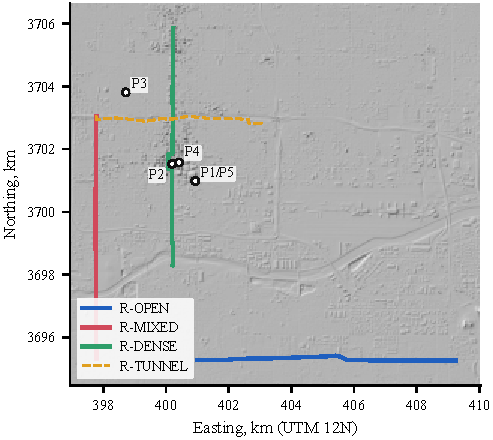
\includegraphics[width=\columnwidth]{fig_aoi.pdf}
\caption{Routes and parking sites over a hillshade of the DSM (UTM zone 12N). P5 is the P1 stall under a modelled shade roof.}
\label{fig:aoi}
\end{figure}

\subsection{Routes, Traffic and Parking Sites}
Routes were chosen by a fixed rule from \RouteCandidates{} candidate \SI{8}{km} windows on the named arterials: the highest mean SVF (R-OPEN, Southern Avenue, SVF \RouteOpenSvf), the lowest (R-DENSE, Central Avenue through downtown, \RouteDenseSvf) and the highest SVF variance in the middle band (R-MIXED, 19th Avenue, \RouteMixedSvf). SUMO~\cite{ref_sumo} on an OpenStreetMap network produced \PsixTraces{} ego traces at \SI{1}{Hz}: both directions, five departures from 08:00 to 16:00 and three traffic demands. The five parking sites (Table~\ref{tab:sites}) span an open lot (P1), a curb in the downtown canyon (P2), a residential driveway beside a tree (P3), a garage roof deck (P4) and the P1 stall under a \SI{4}{m}$\times$\SI{3}{m} shade roof (P5).

\subsection{Shading Engines}
The raster engine marches horizons through the DSM in 360 azimuths at \SI{0.5}{\degree} elevation steps out to \SI{1}{km}, once with trees transparent and once with trees opaque, and corrects azimuths for meridian convergence. Beam visibility of a sample is 1 when lit, 0 behind a building and $\tau=0.03$ behind a tree. The mesh engine casts Embree rays~\cite{ref_embree} against the meshes. Sun positions come from the NREL SPA algorithm~\cite{ref_spa} in pvlib~\cite{ref_pvlib}. The two engines and SOLWEIG were verified in \EoneTotal{} checks covering sun position, transposition, shadow length and canyon SVF; all passed (Table~\ref{tab:valid}).

\section{Vehicle Skin and Energy Chain}
\label{sec:vehicle}
The intended panel layout of the vehicle is not fixed, so we use an assumed design layout (Fig.~\ref{fig:facets}) that totals the conference \SI{11.6}{m^2}: roof \SI{4.4}{m^2} at \SI{2}{\degree}, hood \SI{1.6}{m^2} at \SI{10}{\degree}, tailgate \SI{0.6}{m^2} at \SI{60}{\degree} and two sides of \SI{2.5}{m^2} at \SI{85}{\degree}. Like the mass audit, it is a design estimate; the roof alone is reported as a bound. Each facet is sampled on a \SI{0.25}{m} grid. With the Perez model~\cite{ref_perez} split into beam (with circumsolar) $G_b$, isotropic $G_d$ and horizon $G_h$ components and ground reflection $G_g$ (albedo 0.2), facet $f$ receives
\begin{equation}
G_f=\bar v_{b,f}\,G_{b,f}+\mathrm{SVF}_f\,G_{d,f}+\bar v_{h,f}\,G_{h,f}+G_{g,f},
\label{eq:gf}
\end{equation}
where $\bar v_{b,f}$ is the mean beam visibility of its samples, $\mathrm{SVF}_f$ the cosine-weighted sky view and $\bar v_{h,f}$ the view of the horizon band; all three are 1 in open sky and the sky terms are 0 on covered road. Cell temperature follows Faiman~\cite{ref_faiman}, $T_c=T_a+G_f/(u_0+u_1 w)$ with pvlib's open-rack coefficients and $w$ the wind plus the vehicle speed, and energy follows~\eqref{eq:pv} with $G_f$ for $G$.

\begin{figure}[t]
\centering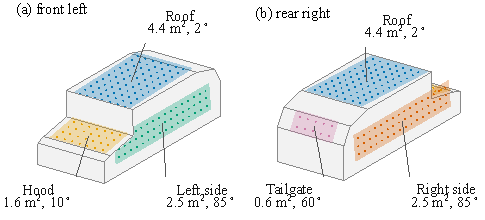
\includegraphics[width=\columnwidth]{fig_facets.pdf}
\caption{Assumed design layout of the \SI{11.6}{m^2} skin with the \SI{0.25}{m} shading samples (area and tilt per facet).}
\label{fig:facets}
\end{figure}

Partial shade costs more electrically than its area suggests. Each facet is one module on its own MPPT input, its samples are cells, and the cells form three bypass-diode substrings. The current--voltage curves come from pvlib's implementation of Bishop's model~\cite{ref_bishop} with reverse breakdown, using area-scaled parameters of a 22.1\%-efficient back-contact cell. Under uniform light the string reproduces the averaged model within \EsixUniform. Over all R-DENSE trips and the P2 and P3 parking steps, the mismatch factor $\Fmm=P_{\mathrm{el}}/P_{\mathrm{avg}}$ is fitted against the beam-shaded fraction $s$ of the facet (Fig.~\ref{fig:fmm}):
\begin{equation}
\Fmm=1-\EsixK\,s^{\EsixAlpha}(1-s)^{\EsixBeta},\qquad R^2=\EsixRsq.
\label{eq:fmm}
\end{equation}
One shaded cell already pushes its substring through the bypass diode, so $\Fmm$ drops steeply at small $s$.

\begin{figure}[t]
\centering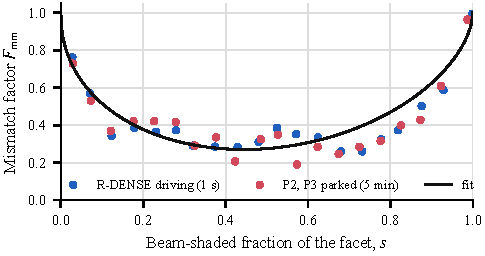
\includegraphics[width=\columnwidth]{fig_fmm.pdf}
\caption{Electrical mismatch factor against the beam-shaded fraction of a facet (energy-weighted bin means) and the fit~\eqref{eq:fmm}.}
\label{fig:fmm}
\end{figure}

Four daily-use archetypes keep the demand of their baseline scenario and change only where the car is when the sun shines. A1, a suburban commuter, drives R-MIXED and R-OPEN at 08:00 and 17:00 and parks at the open lot P1 by day and the driveway P3 at night. A2 and A3 drive R-DENSE and R-OPEN at the same hours and park downtown, at the canyon curb P2 (A2) or under the shade roof P5 (A3). A4, a fleet vehicle, drives \SI{100}{km/day} on all three routes at 08:00 to 16:00 and alternates P2 and P1 between trips. Weekend daytime parking moves to the night site. Parked energy averages the headings that fit each site. Driving at \SI{1}{s} and parking at \SI{5}{min} are binned into the 8760~h of the conference loop; binned and fine energies agree to \EfiveBalance{} and driving plus parked seconds make 3600 in every hour.

\section{Results}
\label{sec:results}
\subsection{Facet Orientation}
Laid flat through the new chain, the skin reproduces the conference harvest within \EtwoIIGate\% (target $\pm0.5\%$); Faiman cooling adds \EtwoIIThermal\%. Averaged over headings, the roof and hood see \FacetRoofGhi{} and \FacetHoodGhi{} of GHI, the tailgate \FacetTailgateGhi{} and the sides \FacetSideLeftGhi. Facet orientation alone lowers $\fss$ from \EtwoIITwoa{} to \EtwoIITwoc{} ($\Fgeo=\EtwoFgeo$) and raises grid charges from \EtwoIIChargesTwoa{} to \EtwoIIChargesTwoc{} per year. The roof alone would give \EtwoIITwod.

\subsection{Driving and Parking Shade}
Table~\ref{tab:sites} lists the shading factors of the \EthreeTrips{} trips and five sites on the TMY. While driving, buildings leave \EthreeOpenB{} of the open-sky harvest on R-OPEN and \EthreeDenseB{} on R-DENSE, and street trees take slightly more. Shading is strongest at the 08:00 and 16:00 departures, when the sun is low, and on R-DENSE the December noon trips also lose far more than the noon trips of the other dates (Fig.~\ref{fig:tod}). Parking spans a much wider range: annual $\Fpark$ is \EfourPOne{} at the open lot, \EfourPThree{} beside the tree and \EfourPTwo{} at the canyon curb, and the shade roof leaves \EfourPFive. Against SOLWEIG the parked shadow maps agree on at least \EfourSolweigLo\% of pixels. The driving losses fall within the 25\% that Brito \emph{et al.}~\cite{ref_brito} found for Lisbon roads, and the curb and driveway losses lie between the Berlin quartiles of Hoth \emph{et al.}~\cite{ref_hoth}.

\begin{figure}[t]
\centering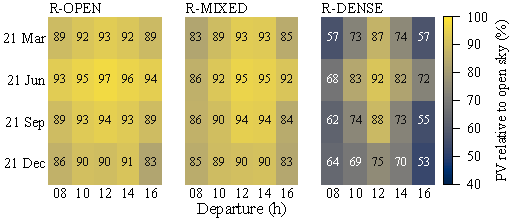
\includegraphics[width=\columnwidth]{fig_tod.pdf}
\caption{Driving PV energy relative to open sky by departure time and date (buildings and trees, TMY, mean of both directions and three traffic demands).}
\label{fig:tod}
\end{figure}

\begin{table}[t]
\caption{Routes and Parking Sites: PV Energy Relative to Open Sky}
\label{tab:sites}
\centering\footnotesize
\begin{tabular}{@{}lccccc@{}}
\toprule
Route & Length & SVF & Buildings & + trees & Beam \\
 & (km) & & $B/A$ & $C/A$ & shaded \\
\midrule
R-OPEN  & \RouteOpenLen  & \RouteOpenSvf  & \EthreeOpenB  & \EthreeOpenCZeroZeroThree  & \EthreeOpenCZeroZeroThreeShaded\% \\
R-MIXED & \RouteMixedLen & \RouteMixedSvf & \EthreeMixedB & \EthreeMixedCZeroZeroThree & \EthreeMixedCZeroZeroThreeShaded\% \\
R-DENSE & \RouteDenseLen & \RouteDenseSvf & \EthreeDenseB & \EthreeDenseCZeroZeroThree & \EthreeDenseCZeroZeroThreeShaded\% \\
\midrule
Site & \multicolumn{2}{c}{Setting} & SVF & $\Fpark$ & \\
\midrule
P1 & \multicolumn{2}{l}{open lot}          & \SitePOneSvf   & \EfourPOne   & \\
P2 & \multicolumn{2}{l}{canyon curb}       & \SitePTwoSvf   & \EfourPTwo   & \\
P3 & \multicolumn{2}{l}{driveway, tree}    & \SitePThreeSvf & \EfourPThree & \\
P4 & \multicolumn{2}{l}{garage roof deck}  & \SitePFourSvf  & \EfourPFour  & \\
P5 & \multicolumn{2}{l}{P1 under shade roof} & ---          & \EfourPFive  & \\
\bottomrule
\end{tabular}\\[2pt]
{\footnotesize Driving: \EthreeTrips{} trips on the TMY days (four dates, both directions, five departures, three demands), trees at $\tau=0.03$. Parking: annual, heading-averaged.}
\end{table}

\subsection{Annual Loss Waterfall}
Fig.~\ref{fig:waterfall} and Table~\ref{tab:annual} carry the baseline to each archetype one correction at a time. The archetype trip hours and the Perez--Faiman chain raise $\fss$ slightly (A1: \EfiveAOneBZero{} to \EfiveAOneChain). Facets then remove \EfiveAOneFacetsDrop{} for the \SI{50}{km} archetypes. Parking shade is the largest and most variable step: \EfiveAOneParkingDrop{} for the commuter, \EfiveAThreeParkingDrop{} under the shade roof and \EfiveATwoParkingDrop{} at the canyon curb. Driving past buildings costs \EfiveAOneBuildingsDrop{} to \EfiveATwoBuildingsDrop, and street trees \EfiveATwoTreesDrop{} or less. Electrical mismatch costs \EfiveAOneMismatchDrop{} to \EfiveAThreeMismatchDrop. Energy-weighted, $\Fmm$ is \EsixDriving{} on the R-DENSE trips and \EsixPtwo{} at the curb, where whole facets fall into building shadow, but \EsixPthreeLo{} to \EsixPthreeHi{} in the dappled shade of the tree at P3. In total the archetypes lose \EfiveAOneLoss\% (A1) to \EfiveATwoLoss\% (A2) of the baseline $\fss$, and grid charges rise from \EfiveAOneBZeroCharges{} to between \EfiveAOneMismatchCharges{} and \EfiveATwoMismatchCharges{} a year. Replacing the hourly TMY with 2023 weather at \SI{5}{min} changes final $\fss$ by at most \EfiveAOneYearEffect, so hourly weather suffices for annual totals.

\begin{figure}[t]
\centering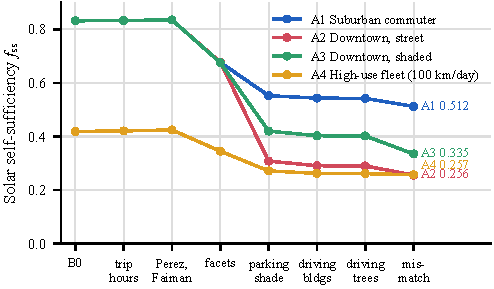
\includegraphics[width=\columnwidth]{fig_waterfall.pdf}
\caption{Annual $\fss$ from the baseline (B0) to each archetype, one correction at a time (Phoenix, TMY).}
\label{fig:waterfall}
\end{figure}

\begin{table}[t]
\caption{Annual Results per Archetype (Phoenix, TMY)}
\label{tab:annual}
\centering\footnotesize
\setlength{\tabcolsep}{3.5pt}
\begin{tabular}{@{}lcccccc@{}}
\toprule
 & \multicolumn{2}{c}{$\fss$} & Loss & Charges/yr & Relief & Grid \\
\cmidrule(lr){2-3}
Archetype & B0 & final & (\%) & B0$\to$final & (\%) & (kWh/yr) \\
\midrule
A1 commuter     & \EfiveAOneBZero   & \EfiveAOneMismatch   & \EfiveAOneLoss   & \EfiveAOneBZeroCharges$\to$\EfiveAOneMismatchCharges     & \EfiveAOneMismatchRelief   & \EfiveAOneMismatchGrid \\
A2 street       & \EfiveATwoBZero   & \EfiveATwoMismatch   & \EfiveATwoLoss   & \EfiveATwoBZeroCharges$\to$\EfiveATwoMismatchCharges     & \EfiveATwoMismatchRelief   & \EfiveATwoMismatchGrid \\
A3 shade roof   & \EfiveAThreeBZero & \EfiveAThreeMismatch & \EfiveAThreeLoss & \EfiveAThreeBZeroCharges$\to$\EfiveAThreeMismatchCharges & \EfiveAThreeMismatchRelief & \EfiveAThreeMismatchGrid \\
A4 fleet        & \EfiveAFourBZero  & \EfiveAFourMismatch  & \EfiveAFourLoss  & \EfiveAFourBZeroCharges$\to$\EfiveAFourMismatchCharges   & \EfiveAFourMismatchRelief  & \EfiveAFourMismatchGrid \\
\bottomrule
\end{tabular}\\[2pt]
{\footnotesize A1--A3: \SI{50}{km/day}, city cycle; A4: \SI{100}{km/day}, full cycle. Loss: share of the B0 $\fss$.}
\end{table}

\section{Shading-Aware Design Inversion}
\label{sec:design}
The waterfall suggests three factors that the conference design equation lacks. From the annual harvest of each archetype at successive steps, $\Fgeo=E_{\mathrm{facets}}/E_{\mathrm{flat}}$, $\Fsh=E_{\mathrm{shaded}}/E_{\mathrm{facets}}$ (parking and driving, weighted by where the car actually is) and $\Fmm=E_{\mathrm{final}}/E_{\mathrm{shaded}}$, and
\begin{equation}
A_{\mathrm{req}}=\frac{D\,c+E_{\mathrm{aux}}}{\eta_{\mathrm{pv}}\,\mathrm{PSH}\,\kappa_{\mathrm{pv}}\,f_T\,\Fgeo\,\Fsh\,\Fmm}.
\label{eq:areqx}
\end{equation}
To test it, the per-facet harvest of each archetype was recomputed and scaled to other areas and allocations (roof only, roof and hood, full skin, with the area spread over the allocated facets in proportion), and the hour-by-hour simulation, with the vehicle mass fed back at \SI{3.5}{kg/m^2}, was solved for the area at which $\fss=1$. Over \EsevenN{} cases (four archetypes, three allocations, $\kappa_{\mathrm{pv}}=0.60$ to 0.80) \eqref{eq:areqx} stays within \EsevenMaxErr\% of the simulation (\EsevenMaxErrFixed\% with the mass held fixed), inside the 3\% target. Table~\ref{tab:design} lists the factors for the full skin and Fig.~\ref{fig:nomo} the resulting design curves.

\begin{table}[t]
\caption{Loss Factors and Required Area (Full Skin, $\kappa_{\mathrm{pv}}=0.80$)}
\label{tab:design}
\centering\footnotesize
\setlength{\tabcolsep}{3.2pt}
\begin{tabular}{@{}lccccccc@{}}
\toprule
 & $\Fgeo$ & $\Fsh$ & $\Fmm$ & \multicolumn{2}{c}{$A_{\mathrm{req}}$ (\si{m^2})} & Error & $D_{\max}$ \\
\cmidrule(lr){5-6}
 & & & & \eqref{eq:areqx} & sim. & (\%) & (km/d) \\
\midrule
A1 & \EsevenAOneFullSkinFgeo   & \EsevenAOneFullSkinFsh   & \EsevenAOneFullSkinFmm   & \EsevenAOneAreq   & \EsevenAOneAsim   & \EsevenAOneErr   & \EsevenAOneDmax \\
A2 & \EsevenATwoFullSkinFgeo   & \EsevenATwoFullSkinFsh   & \EsevenATwoFullSkinFmm   & \EsevenATwoAreq   & \EsevenATwoAsim   & \EsevenATwoErr   & \EsevenATwoDmax \\
A3 & \EsevenAThreeFullSkinFgeo & \EsevenAThreeFullSkinFsh & \EsevenAThreeFullSkinFmm & \EsevenAThreeAreq & \EsevenAThreeAsim & \EsevenAThreeErr & \EsevenAThreeDmax \\
A4 & \EsevenAFourFullSkinFgeo  & \EsevenAFourFullSkinFsh  & \EsevenAFourFullSkinFmm  & \EsevenAFourAreq  & \EsevenAFourAsim  & \EsevenAFourErr  & \EsevenAFourDmax \\
\bottomrule
\end{tabular}\\[2pt]
{\footnotesize B0 for comparison: $A_{\mathrm{req}}=\BzPhxIIAreq$ (Scen.~II) and \BzPhxIAreq{} \si{m^2} (Scen.~I). $D_{\max}$ at \SI{11.6}{m^2}.}
\end{table}

\begin{figure*}[t]
\centering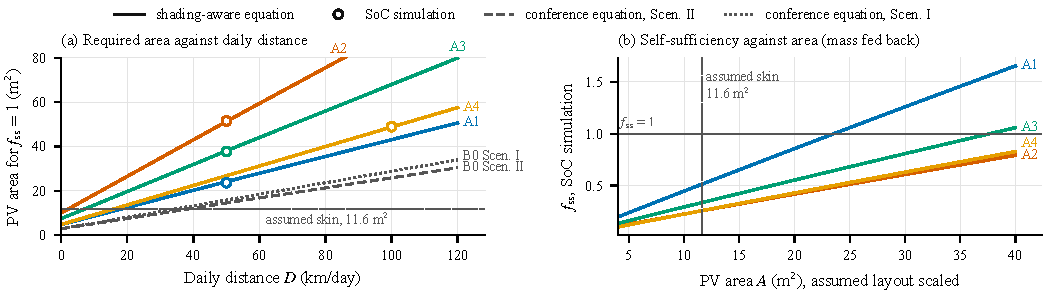
\includegraphics[width=\textwidth]{fig_nomograph.pdf}
\caption{(a) Area for $\fss=1$ against daily distance from~\eqref{eq:areqx} for each archetype (full skin, $\kappa_{\mathrm{pv}}=0.80$), with the hour-by-hour simulation (circles) and the conference equation~\eqref{eq:areq} (gray). (b) $\fss$ against area in the simulation.}
\label{fig:nomo}
\end{figure*}

On the full skin, a commuter would need \EsevenAOneAreq{}~\si{m^2} instead of \BzPhxIIAreq{}~\si{m^2}, and a downtown street parker \EsevenATwoAreq{}~\si{m^2}, more than the roof, hood and sides of the vehicle can hold. Put the other way, the \SI{11.6}{m^2} skin covers \EsevenAOneDmax{}~km/day for the commuter against \BzPhxIIDmax{}~km/day in the baseline. A roof-only skin of the same area would have a higher $\Fgeo$ but does not fit on the roof; the sweep table in the repository gives $\fss$ for every area, allocation, $\kappa_{\mathrm{pv}}$ and archetype.

\section{Validation of the Twin}
\label{sec:validation}
Without measured on-vehicle irradiance, the twin is cross-verified rather than physically validated (Table~\ref{tab:valid}, Fig.~\ref{fig:valid}). Unity~6 with Cesium for Unity imported the same meshes around R-DENSE, replayed all \EeightTrips{} trip-dates and cast PhysX rays from every sample once per second. Its surface lies within \EeightMarksMax{}~m of the lidar at \EeightMarksN{} survey marks. Unity and the raster engine agree on \EeightAgree\% of \EeightRecords~million sample-seconds; trip lit fractions agree within 2 percentage points (pp) on \EeightWithin{} of \EeightTrips{} trips (largest \EeightMaxPp~pp). Embree on the same meshes reproduces Unity to \EeightEmbreeMaxPp~pp, which locates the remaining difference in the surface representation: the raster treats each pixel as a flat-topped column, while the mesh rounds roof edges. The \SI{\pm1}{\degree} band around the horizon line holds \EeightBandShare\% of sample-seconds but \EeightBandDis\% of disagreements; outside it every trip agrees within \EeightBeyondMaxPp~pp.

Mapillary panoramas~\cite{ref_mapillary} within \SI{10}{m} of R-DENSE and R-MIXED and at least \SI{250}{m} apart give \EeightSvfAllN{} test points. Their sky segmentation gives SVF with the engine's cosine weighting. Of these, \EeightSvfKeptN{} agree with MAE \EeightSvfKeptMae{} and $r=\EeightSvfKeptR$; the remaining panorama was taken on an overpass deck that the route passes beneath, where the engine correctly sees the deck (all \EeightSvfAllN: MAE \EeightSvfAllMae). With so few points this is a plausibility check.

\begin{figure}[t]
\centering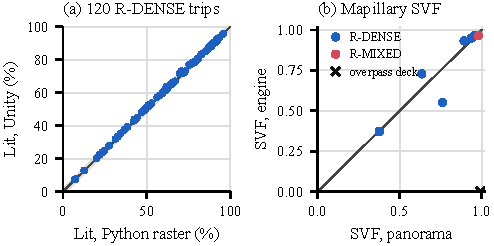
\includegraphics[width=\columnwidth]{fig_validation.pdf}
\caption{(a) Trip lit fraction, Unity against the raster engine (band $\pm2$~pp). (b) SVF from Mapillary panoramas against the engine at \SI{2}{m}.}
\label{fig:valid}
\end{figure}

\begin{table}[t]
\caption{Verification and Validation Metrics}
\label{tab:valid}
\centering\footnotesize
\setlength{\tabcolsep}{3pt}
\begin{tabular}{@{}p{0.47\columnwidth}cc@{}}
\toprule
Check & Result & Target \\
\midrule
Engine checks (sun, transposition, shadows, SVF) & \EonePassed/\EoneTotal & all \\
Raster vs.\ mesh beam, 1000 points, 43 suns & \EoneBeam\% & $\ge98\%$ \\
Raster vs.\ mesh SVF, mean $|\Delta|$ & \EoneDsvf & $<0.02$ \\
SOLWEIG shadow pixels, 12 times & \EoneSolweigLo--\EoneSolweigHi\% & $\ge95\%$ \\
SOLWEIG at parking sites & $\ge$\EfourSolweigLo\% & $\ge95\%$ \\
Unity vs.\ raster, sample-seconds & \EeightAgree\% & $\ge97\%$ \\
Unity vs.\ raster, trips within 2~pp & \EeightWithin/\EeightTrips & all \\
Mapillary SVF, MAE ($n=\EeightSvfKeptN$) & \EeightSvfKeptMae & reported \\
Energy closure, all steps & $\EfiveBalance$ & $\le10^{-3}$ \\
\bottomrule
\end{tabular}
\end{table}

\begin{figure}[t]
\centering
\fbox{\parbox{0.92\columnwidth}{\centering\footnotesize\textbf{[Figure placeholder: Unity render]}\\[2pt]
R-DENSE northbound, 21 December, 08:00 departure, medium traffic, analysis geometry in shadows-only mode under Google Photorealistic 3D Tiles. Scene as specified in PAPER\_CHANGELOG.md (P8). Rendered by the authors.\\[16mm]}}
\caption{The Unity twin on R-DENSE on a winter morning, with the shadow on the skin from the analysis geometry. Imagery: Google; Cesium.}
\label{fig:render}
\end{figure}

\section{Discussion and Limitations}
\label{sec:discussion}
Where the car parks matters more than where it drives: the commuter keeps \EfiveAOneMismatch{} because it parks in the open by day, while the same vehicle with the same trips keeps \EfiveATwoMismatch{} at a downtown curb. For design, \eqref{eq:areqx} turns a site survey into three multiplicative factors that can be estimated from shade maps without a full simulation, and the error of the closed form is smaller than the spread between archetypes.

The method transfers to other cities. London's PVGIS weather is already in Table~\ref{tab:b0}; the geometry needs national lidar (the Environment Agency survey in England) and the same building and street sources. A lower sun and narrower streets would likely raise the parking and orientation losses there, so the London baseline of \BzLonIIfss{} should be read as an upper bound.

The limitations are as follows. The panel layout is an assumed design; side panels dominate $\Fgeo$, so a roof-heavy design would lose less to orientation. Mismatch depends on the module layout (three diodes per facet module and \SI{0.25}{m} cells); more diodes or per-substring tracking would reduce it. Trees use one transmissivity and the lidar canopy of 2020, without seasonal leaf change. Traffic is simulated and the arterials stay below saturation, so queues in shade are underrepresented. The weather is a typical year, the shading and SVF were verified against models and imagery rather than measured irradiance on a vehicle, and \FreshUnreviewed{} smaller building changes along the routes were not reviewed.

\section{Conclusion}
A digital twin of central Phoenix shows that the usual horizontal, unshaded roof overstates the solar self-sufficiency of a heavy VIPV vehicle: the four archetypes lose \EfiveAOneLoss\% to \EfiveATwoLoss\% of the baseline value. Starting from \BzPhxIIfss{} at \SI{50}{km/day}, facet orientation and shade leave \EfiveAOneMismatch{} for a suburban commuter and \EfiveATwoMismatch{} for a car parked at a downtown curb, and grid charges rise from \EfiveAOneBZeroCharges{} to \EfiveAOneMismatchCharges--\EfiveATwoMismatchCharges{} a year. Parking shade is the largest loss after orientation; driving through street canyons costs at most \EfiveATwoBuildingsDrop. A shading-aware design equation reproduces the full simulation within \EsevenMaxErr\% and gives the required area for a new site from three factors.

\section*{Code and Data Availability}
The pipeline, configuration, frozen route manifest and result tables are at \url{https://github.com/jarvisxys/solaris-vipv}; the conference toolkit is at \url{https://github.com/Anandsagar18/Solaris}~\cite{ref_code}. Lidar, NAIP and NSRDB data are public and fetched by the pipeline; Overture and OpenStreetMap data are under ODbL and Mapillary imagery under CC BY-SA 4.0.

\section*{Acknowledgment}
\emph{Use of generative AI.} Following IEEE policy, the authors disclose that Claude (Anthropic) was used to help write, refactor and debug the analysis code and to help draft and edit the manuscript text. The study design, modeling choices, interpretation and conclusions are the authors'. The authors reviewed and edited all AI-assisted code and text, every number in the paper is generated by the released pipeline, and the authors take full responsibility for the content.

\begin{thebibliography}{99}
\footnotesize
\bibitem{ref_conf} A.~Gaikwad, A.~Kumar, and A.~Deo, ``SOLARIS: A first-principles, drive-cycle- and climate-resolved methodology and open toolkit for assessing solar-assisted heavy electric vehicles,'' accepted for presentation at the \emph{IEEE Transp.\ Electrific.\ Conf.\ Expo, Asia-Pacific (ITEC-AP 2026)}, Busan, Republic of Korea, Dec.\ 2026.
\bibitem{ref_code} A.~Gaikwad, A.~Kumar, and A.~Deo, ``SOLARIS: An open toolkit for solar-assisted heavy EV feasibility assessment,'' version~1.1.0, 2026. [Online]. Available: \url{https://github.com/Anandsagar18/Solaris}
\bibitem{ref_commault} B.~Commault, T.~Duigou, V.~Maneval, J.~Gaume, F.~Chabuel, and E.~Voroshazi, ``Overview and perspectives for vehicle-integrated photovoltaics,'' \emph{Appl.\ Sci.}, vol.~11, no.~24, Art.~no.~11598, Dec.\ 2021, doi: 10.3390/app112411598.
\bibitem{ref_samadi} H.~Samadi, G.~Ala, V.~Lo~Brano, P.~Romano, and F.~Viola, ``Investigation of effective factors on vehicles integrated photovoltaic (VIPV) performance: A review,'' \emph{World Electr.\ Veh.\ J.}, vol.~14, no.~6, Art.~no.~154, Jun.\ 2023, doi: 10.3390/wevj14060154.
\bibitem{ref_carr} A.~J.~Carr \emph{et al.}, ``Solar Moves: Part 1, modelling the impact of VIPV,'' \emph{Sol.\ Energy Mater.\ Sol.\ Cells}, vol.~275, Art.~no.~113023, Sep.\ 2024, doi: 10.1016/j.solmat.2024.113023.
\bibitem{ref_sanjose} L.~San~Jos\'e, R.~Moruno, R.~N\'u\~nez, R.~Herrero, J.~Mac\'ias, and I.~Ant\'on, ``Performance evaluation of MPPT algorithm of VIPV systems in realistic urban routes using image processing,'' \emph{Sol.\ Energy Mater.\ Sol.\ Cells}, vol.~276, Art.~no.~113061, Oct.\ 2024, doi: 10.1016/j.solmat.2024.113061.
\bibitem{ref_yavasoglu} H.~Yavasoglu, B.~Shani, A.~Hasnain, B.~Parlak, and A.~Khaligh, ``Analysis and system design optimization of PV panel and auxiliary battery integration for VIPV electric vehicles,'' \emph{IEEE Trans.\ Transport.\ Electrific.}, vol.~11, no.~6, pp.~13535--13545, Dec.\ 2025, doi: 10.1109/TTE.2025.3600891.
\bibitem{ref_brito} M.~C.~Brito, T.~Santos, F.~Moura, D.~Pera, and J.~Rocha, ``Urban solar potential for vehicle integrated photovoltaics,'' \emph{Transp.\ Res.\ Part D: Transp.\ Environ.}, vol.~94, Art.~no.~102810, May 2021, doi: 10.1016/j.trd.2021.102810.
\bibitem{ref_hoth} P.~Hoth, L.~Heide, A.~Grahle, and D.~G\"ohlich, ``Vehicle-integrated photovoltaics---A case study for Berlin,'' \emph{World Electr.\ Veh.\ J.}, vol.~15, no.~3, Art.~no.~113, Mar.\ 2024, doi: 10.3390/wevj15030113.
\bibitem{ref_middel} A.~Middel, J.~Lukasczyk, and R.~Maciejewski, ``Sky view factors from synthetic fisheye photos for thermal comfort routing---A case study in Phoenix, Arizona,'' \emph{Urban Planning}, vol.~2, no.~1, pp.~19--30, 2017, doi: 10.17645/up.v2i1.855.
\bibitem{ref_solweig} F.~Lindberg, B.~Holmer, and S.~Thorsson, ``SOLWEIG 1.0---Modelling spatial variations of 3D radiant fluxes and mean radiant temperature in complex urban settings,'' \emph{Int.\ J.\ Biometeorol.}, vol.~52, no.~7, pp.~697--713, 2008, doi: 10.1007/s00484-008-0162-7.
\bibitem{ref_umep} F.~Lindberg \emph{et al.}, ``Urban Multi-scale Environmental Predictor (UMEP): An integrated tool for city-based climate services,'' \emph{Environ.\ Model.\ Softw.}, vol.~99, pp.~70--87, Jan.\ 2018, doi: 10.1016/j.envsoft.2017.09.020.
\bibitem{ref_nsrdb} M.~Sengupta, Y.~Xie, A.~Lopez, A.~Habte, G.~Maclaurin, and J.~Shelby, ``The National Solar Radiation Data Base (NSRDB),'' \emph{Renew.\ Sustain.\ Energy Rev.}, vol.~89, pp.~51--60, Jun.\ 2018, doi: 10.1016/j.rser.2018.03.003.
\bibitem{ref_pvgis} European Commission Joint Research Centre, ``Photovoltaic Geographical Information System (PVGIS) 5.3, typical meteorological year, PVGIS-SARAH3, 2005--2023.'' [Online]. Available: \url{https://re.jrc.ec.europa.eu/pvg_tools/en/}
\bibitem{ref_3dep} U.S. Geological Survey, ``3D Elevation Program lidar point cloud, AZ\_MaricopaPinal\_2020\_B20,'' Entwine point tiles on AWS Open Data. [Online]. Available: \url{https://registry.opendata.aws/usgs-lidar/}
\bibitem{ref_naip} U.S. Department of Agriculture Farm Service Agency, ``National Agriculture Imagery Program (NAIP), Arizona 2021,'' via Microsoft Planetary Computer. [Online]. Available: \url{https://planetarycomputer.microsoft.com/dataset/naip}
\bibitem{ref_overture} Overture Maps Foundation, ``Buildings theme, release 2026-09-23.1.'' [Online]. Available: \url{https://overturemaps.org}
\bibitem{ref_osm} OpenStreetMap contributors, ``OpenStreetMap.'' [Online]. Available: \url{https://www.openstreetmap.org}
\bibitem{ref_sumo} P.~A.~Lopez \emph{et al.}, ``Microscopic traffic simulation using SUMO,'' in \emph{Proc.\ 21st IEEE Int.\ Conf.\ Intell.\ Transp.\ Syst.\ (ITSC)}, 2018, pp.~2575--2582, doi: 10.1109/ITSC.2018.8569938.
\bibitem{ref_embree} I.~Wald, S.~Woop, C.~Benthin, G.~S.~Johnson, and M.~Ernst, ``Embree: A kernel framework for efficient CPU ray tracing,'' \emph{ACM Trans.\ Graph.}, vol.~33, no.~4, Art.~no.~143, 2014, doi: 10.1145/2601097.2601199.
\bibitem{ref_spa} I.~Reda and A.~Andreas, ``Solar position algorithm for solar radiation applications,'' \emph{Sol.\ Energy}, vol.~76, no.~5, pp.~577--589, 2004, doi: 10.1016/j.solener.2003.12.003.
\bibitem{ref_pvlib} K.~S.~Anderson \emph{et al.}, ``pvlib python: 2023 project update,'' \emph{J.\ Open Source Softw.}, vol.~8, no.~92, Art.~no.~5994, 2023, doi: 10.21105/joss.05994.
\bibitem{ref_perez} R.~Perez, P.~Ineichen, R.~Seals, J.~Michalsky, and R.~Stewart, ``Modeling daylight availability and irradiance components from direct and global irradiance,'' \emph{Sol.\ Energy}, vol.~44, no.~5, pp.~271--289, 1990, doi: 10.1016/0038-092X(90)90055-H.
\bibitem{ref_faiman} D.~Faiman, ``Assessing the outdoor operating temperature of photovoltaic modules,'' \emph{Prog.\ Photovolt.: Res.\ Appl.}, vol.~16, no.~4, pp.~307--315, 2008, doi: 10.1002/pip.813.
\bibitem{ref_bishop} J.~W.~Bishop, ``Computer simulation of the effects of electrical mismatches in photovoltaic cell interconnection circuits,'' \emph{Solar Cells}, vol.~25, no.~1, pp.~73--89, 1988, doi: 10.1016/0379-6787(88)90059-2.
\bibitem{ref_mapillary} Mapillary, ``Mapillary API v4,'' street-level imagery and semantic segmentation, CC BY-SA 4.0. [Online]. Available: \url{https://www.mapillary.com/developer/api-documentation}
\end{thebibliography}

\end{document}
